
\section{Fairness-for-Event-B}
\label{sec:Fairness-for-Event-B}

% K: fixme

\newcommand{\WF}{\mathrm{WF}}
\newcommand{\SF}{\mathrm{SF}}
\subsection{Introduction}
% K1: all of this is either wrong or imprecise. fix.
Fairness is a property for system which have infinite execution, this property ensure that transitions (events) can be "fairly" chosen to execute when their preconditions (guards) are satisfied. Without fairness constraints, it's possible that some transitions can be always ignored even if they are enabled in some states. It does not make sense to deal with fairness constraints on systems with finite execution.
\paragraph{Weak Fairness}
% K1: none of this makes sense. WF(t) is a quality of an execution (and a transition set t)
An transition set t is a weakly fair set if every transition in t is always eventually disabled or infinitely often taken.
% K1: this doesn't look right. so i fixed it. use it as a blueprint how to do things
% \begin{center}
% WF(i)$\Equiv\Always\Eventually\Not{g}_{i}\Or\Always\Eventually{taken}_{i}$ 
% \end{center}
\begin{displaymath}
  \WF(i)\Equiv\Always\Eventually\Not g_i\Or\Always\Eventually\mathrm{taken}_i
\end{displaymath}

\paragraph{Strong Fairness}
% K1: same as above
An transition set t is a strongly fair set if every transition in t is eventually always disabled or infinitely often taken.
\begin{gather*}
  \SF(i)\Equiv\Eventually\Always\Not g_i\Or\Always\Eventually{\mathrm{taken}}_i
\end{gather*}
% K1: now this sentence scares me. it's the wrong way around! SF => WF
% X: Fixed

However, by working on the definitions for weak fairness and strong fairness, we can easily find that strong fairness imply weak fairness. Strong fairness is stronger than weak fairness.  

\begin{gather*}
  \SF(i)\Implies \WF(i)  % FIXME
\end{gather*}

\paragraph{Event Merging}

For some situations we only have the fairness constraints for a set of events instead of fairness constraints for each of them. For example, Peter wants to travel all over the world, once he arrives at a new place, he might stay there and spend several days for sightseeing. In this example, assume having an one-day sightseeing is modeled as the event $E_{\mathrm{s}}$, and we specify the event $E_{\mathrm{t}}$ as the event of moving to a new place by either of the two offered means of transporation. \\
\setlength\fboxsep{0pt}
\setlength\fboxrule{0pt}
\fbox{    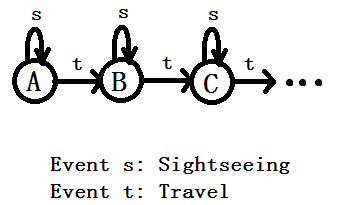
\includegraphics{pics/travel_problem_1.png} }\\
% \graphicspath{ {pics/} }
% \caption{Travel Problem 1}\label{fig:travel_problem_1}
The following constraint
% K1: fix up all formulae similar to what I did to those above
\begin{displaymath}
  \WF(t)
\end{displaymath}
must be satisfied to ensure he does move from one place to another rather than spending the rst of his life sightseeing somewhere without ever moving again.\\
Assume Peter can only use train or aiplane to travel, we replace event $E_{\mathrm{t}}$ by event $E_{\mathrm{air}}$ and event $E_{\mathrm{train}}$, where the event $E_{\mathrm{air}}$ is for moving on air and the event $E_{\mathrm{train}}$ is for moving by train. \\
\fbox{    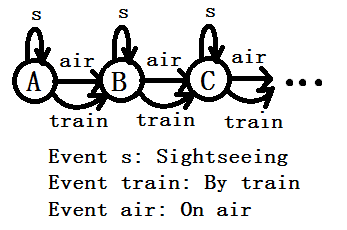
\includegraphics{pics/travel_problem_2.png} }\\
If every place has an airport and a train station, or none of them, travel is fair (can be always eventually chosen) iff air is fair (can be always eventually chosen) or train is fair (can be always eventually chosen). Since if one of the transportations is fair to choose, he can always eventually move to other places.
\begin{displaymath}
  \mathrm{I}\And{g_{air}} = \mathrm{I}\And{g_{train}}\Implies(\WF(travel)\Equiv\WF(air)\lor\WF(train))
\end{displaymath}
However, if there have at least one place that has only have airport, $\WF(train)$ can't ensure he can leave this place unless there have extra requirements force him occationally move on air (weak fairness for air when train is disabled). We also have similar problem for places only have train station. \\
\fbox{    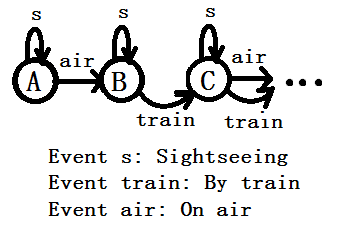
\includegraphics{pics/travel_problem_3.png} }\\
We have:
%X: I wanna say that WF(air at g_{air}\And\Not{g}_{train}
\begin{displaymath}
  (\WF(train)\And\WF(air@g_{air}\And\Not{g}_{train}))\Or(\WF(air)\And\WF(train@g_{train}\And\Not{g}_{air})) \Equiv\WF(t)
\end{displaymath}

% K1: now we have a little problem with this example unless you also make up at least one location that has only an airport or only a train station. Otherwise you end up with  WF(air) \/ WF(train) <=> WF(train\/air).
% X:
For this type of constraints, we introduce the following rule for
merging events: For event $E_{i}$ and event $E_{j}$, where $i,j \in$
I, the merged event $E_{i\Or j}$ is given as:
\begin{align*}
g_{i\Or {j}} & =  g_i\Or g_j\\
a_{i\Or {j}} & |  a'_{i\Or j} \And \\
           &    (((g_i\And\Not g_j)\Implies (a'_{i\Or j} = a_i))\\
           &    \Or ((\Not g_i\And g_j)\Implies (a'_{i\Or j} = a_j))\\
           &    \Or ((g_i\And g_j)\Implies (a'_{i\Or j} = a_j\Or a_j)))
\end{align*}
% K1: this following explanation fails. Say that the merged event can happen whenever either of its constituent events could fire, and if it fires, the effect is one of the enabled constituent events.
The merged event $E_{i\lor{j}}$ can happen whenever either of its constituent events ($E_i$ and $E_j$) could fire, and if $E_{i\lor{j}}$ fires, the effect is one of the enabled constituent events.\\
Some properties for fairness constraints of merged events are:\\
Assume $i,j \in$ I, event $E_{i\Or j}$ is the result of merging events $E_i$ and $E_j$.
\begin{gather*} 
  (\WF(i)\And\WF(j@g_{j}\And\Not{g}_{i}))\Or(\WF(j)\And\WF(i@g_{i}\And\Not{g}_{j})) \Equiv\WF(i\Or{j})\\
  (\SF(i)\And\SF(j@g_{j}\And\Not{g}_{i}))\Or(\SF(j)\And\SF(i@g_{i}\And\Not{g}_{j})) \Equiv\SF(i\Or{j})
\end{gather*}

\paragraph{Event Splitting}

% K1: "several" means 2 here
In an opposite way, we can also split an event into two mutually exclusive sub-events, by refining them with different mutually exclusive strengthened guards which imply the original guard. \\
For event $h$ where $h \in I$, event $i$ and event $j$ are \emph{split} events of $h$ iff:
\begin{gather*} 
g_i \Or g_j \Equiv g_h\\
\Not(g_i\And g_j)\\
a_i = a_j = a_h
\end{gather*}
Note that the fairness constraints of the original event are not inherited to its sub-events, for the same reason explained in event merging part.
% K1: I don't see how this sentence helps anyone. Since when do parents inherent from their kids?
% X: I wanna say something like the sub-events are not necessary fair when the orginal event is fair. 
However, similar to the outcome of the event merging process, we can say a event is fair if we can ensure that one of its sub-events is fair, since the sub-events have same guard as the original event.
\begin{gather*} 
  \WF(i) \Or \WF(j) \Implies  \WF(h)\\
  \SF(i) \Or \SF(j) \Implies \SF(h)
\end{gather*}
Where event $i$ and $j$ are sub-events of event $h$.\\\\
% K1: you repeat the nonsense about unbounded nondeterminism. FIXME
Currently Event-B does not have suppport for LTL, most of properties described by LTL (including fairness) can't be assumed or proved by Event-B. In the rest parts of this report, we will extend the original Event-B method and show the usage of fairness assumptions for proving response properties.\\


 	$\sideset{_1^2}{_3^4}\prod_a^b$
 	$\bigvee_{i=_1}^n E_i$

%====================